\documentclass[a4paper]{article}
\usepackage{geometry}
\usepackage{graphicx}
\usepackage{natbib}
\usepackage{amsmath}
\usepackage{amssymb}
\usepackage{amsthm}
\usepackage{paralist}
\usepackage{epstopdf}
\usepackage{tabularx}
\usepackage{longtable}
\usepackage{multirow}
\usepackage{multicol}
\usepackage[hidelinks]{hyperref}
\usepackage{fancyvrb}
\usepackage{algorithm}
\usepackage{algorithmic}
\usepackage{float}
\usepackage{paralist}
\usepackage[svgname]{xcolor}
\usepackage{enumerate}
\usepackage{array}
\usepackage{times}
\usepackage{url}
\usepackage{fancyhdr}
\usepackage{comment}
\usepackage{environ}
\usepackage{times}
\usepackage{textcomp}
\usepackage{caption}
\usepackage{color}
\usepackage{xcolor}
\usepackage{subcaption}

\urlstyle{rm}

\setlength\parindent{0pt} % Removes all indentation from paragraphs
\theoremstyle{definition}
\newtheorem{definition}{Definition}[]
\newtheorem{conjecture}{Conjecture}[]
\newtheorem{example}{Example}[]
\newtheorem{theorem}{Theorem}[]
\newtheorem{lemma}{Lemma}
\newtheorem{proposition}{Proposition}
\newtheorem{corollary}{Corollary}

\floatname{algorithm}{Procedure}
\renewcommand{\algorithmicrequire}{\textbf{Input:}}
\renewcommand{\algorithmicensure}{\textbf{Output:}}
\newcommand{\abs}[1]{\lvert#1\rvert}
\newcommand{\norm}[1]{\lVert#1\rVert}
\newcommand{\RR}{\mathbb{R}}
\newcommand{\CC}{\mathbb{C}}
\newcommand{\Nat}{\mathbb{N}}
\newcommand{\br}[1]{\{#1\}}
\DeclareMathOperator*{\argmin}{arg\,min}
\DeclareMathOperator*{\argmax}{arg\,max}
\renewcommand{\qedsymbol}{$\blacksquare$}

\definecolor{dkgreen}{rgb}{0,0.6,0}
\definecolor{gray}{rgb}{0.5,0.5,0.5}
\definecolor{mauve}{rgb}{0.58,0,0.82}

\newcommand{\Var}{\mathrm{Var}}
\newcommand{\Cov}{\mathrm{Cov}}

\newcommand{\vc}[1]{\boldsymbol{#1}}
\newcommand{\xv}{\vc{x}}
\newcommand{\Sigmav}{\vc{\Sigma}}
\newcommand{\alphav}{\vc{\alpha}}
\newcommand{\muv}{\vc{\mu}}

\newcommand{\red}[1]{\textcolor{red}{#1}}

\def\x{\mathbf x}
\def\y{\mathbf y}
\def\w{\mathbf w}
\def\v{\mathbf v}
\def\E{\mathbb E}
\def\V{\mathbb V}

% TO SHOW SOLUTIONS, include following (else comment out):
\newenvironment{soln}{
    \leavevmode\color{blue}\ignorespaces
}{}


\hypersetup{
%    colorlinks,
    linkcolor={red!50!black},
    citecolor={blue!50!black},
    urlcolor={blue!80!black}
}

\geometry{
  top=1in,            % <-- you want to adjust this
  inner=1in,
  outer=1in,
  bottom=1in,
  headheight=3em,       % <-- and this
  headsep=2em,          % <-- and this
  footskip=3em,
}


\pagestyle{fancyplain}
\lhead{\fancyplain{}{Homework 2}}
\rhead{\fancyplain{}{CS 760 Machine Learning}}
\cfoot{\thepage}

\title{\textsc{Homework 2}} % Title

%%% NOTE:  Replace 'NAME HERE' etc., and delete any "\red{}" wrappers (so it won't show up as red)

\author{
\red{$>>$Nevindu M. Batagoda$<<$} \\
\red{$>>$9081677594$<<$}\\
} 

\date{}

\begin{document}

\maketitle 


\textbf{Instructions:} 
Use this latex file as a template to develop your homework. Submit your homework on time as a single pdf file to Canvas. Please wrap your code and upload to a public GitHub repo, then attach the link below the instructions so that we can access it. You can choose any programming language (i.e. python, R, or MATLAB), as long as you implement the algorithm from scratch (e.g. do not use sklearn on questions 1 to 7 in section 2). Please check Piazza for updates about the homework. \\

GitHub repo: \url{https://github.com/Nevindu/CS760.HW2}

\section{A Simplified Decision Tree}
You are to implement a decision-tree learner for classification.
To simplify your work, this will not be a general purpose decision tree.  Instead, your program can assume that
\begin{itemize}
\item each item has two continuous features $\x \in \RR^2$
\item the class label is binary and encoded as $y \in \{0,1\}$
\item data files are in plaintext with one labeled item per line, separated by whitespace:
$$x_{11} \quad x_{12} \quad y_1$$
$$...$$
$$x_{n1} \quad x_{n2} \quad y_n$$
\end{itemize}

Your program should implement a decision tree learner according to the following guidelines:
\begin{itemize}
\item Candidate splits $(j,c)$ for numeric features should use a threshold $c$ in feature dimension $j$ in the form of $x_{j}\ge c$.
\item $c$ should be on values of that dimension present in the training data; i.e. the threshold is on training points, not in between training points. You may enumerate all features, and for each feature, use all possible values for that dimension.
\item You may skip those candidate splits with zero split information (i.e. the entropy of the split), and continue the enumeration.
\item The left branch of such a split is the ``then'' branch, and the right branch is ``else''.
\item Splits should be chosen using information gain ratio. If there is a tie you may break it arbitrarily.
\item The stopping criteria (for making a node into a leaf) are that 
	\begin{itemize}
	\item the node is empty, or
	\item all splits have zero gain ratio (if the entropy of the split is non-zero), or
	\item the entropy of any candidates split is zero
	\end{itemize}
\item To simplify, whenever there is no majority class in a leaf, let it predict $y=1$.
\end{itemize}

\section{Questions}
\begin{enumerate}
\item (Our algorithm stops at pure labels) [10 pts] If a node is not empty but contains training items with the same label, why is it guaranteed to become a leaf?  Explain. You may assume that the feature values of these items are not all the same. \\

  \begin{soln}
    If node only has items of the same class, then the entropy of the split is 0 because the probability of one class is 1 and for the other is 0. Therefore, the information gain ratio is 0 for all possible splits. Therefore, the algorithm will stop at this node and make it a leaf.
  \end{soln}

\item (Our algorithm is greedy)  [10 pts] Handcraft a small training set where both classes are present but the algorithm refuses to split; instead it makes the root a leaf and stop;
Importantly, if we were to manually force a split, the algorithm will happily continue splitting the data set further and produce a deeper tree with zero training error.
You should (1) plot your training set, (2) explain why.  Hint: you don't need more than a handful of items. \\

\begin{soln}
  Consider the following training set,
  \begin{figure}[H]
    \centering
    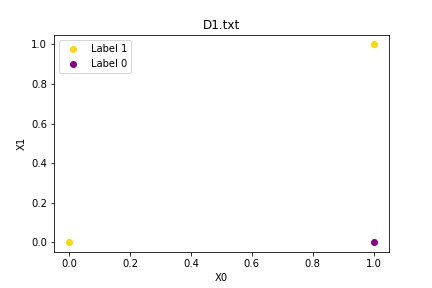
\includegraphics[width=0.5\textwidth]{hand_scatter.jpg}
    \caption{Example of when the algorithm stops at the root node and refuses to split}
    \label{fig:q2_1}
  \end{figure}

  Since we split on feature values, and data points from two classes lie on the same line the algorithm cannot cleanly split this training set. However, if we force the algorithm to split it will create a complicated tree with more nodes than training points as in the following Figure.(\ref{fig:q2_2}).

  \begin{figure}[H]
    \centering
    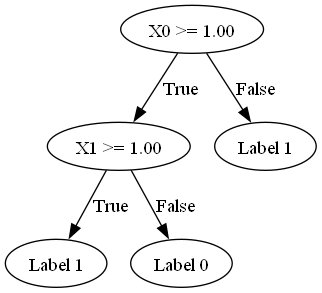
\includegraphics[width=5cm]{hand_vis.png}
    \caption{Decision tree for the training set in Figure.(\ref{fig:q2_1})}
    \label{fig:q2_2}
  \end{figure}
\end{soln}


\item (Information gain ratio exercise)  [10 pts] Use the training set Druns.txt.  For the root node, list all candidate cuts and their information gain ratio. If the entropy of the candidate split is zero, please list its mutual information (i.e. information gain). Hint: to get $\log_2(x)$ when your programming language may be using a different base, use \verb|log(x)/log(2)|. Also, please follow the split rule in the first section. \\

\begin{soln}
  The following Figure.(\ref{fig:q2_3}) shows all the candidates for features $x_0$ and $x_1$ and their information gain ratio. \\
    \begin{figure}[H]
      \centering
      \begin{subfigure}[b]{0.3\textwidth}
          \centering
          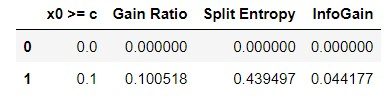
\includegraphics[width=\textwidth]{q2_3_x0.jpg}
          \caption{Information gain ratio for feature $x_0$}
          \label{fig:ig_x0}
      \end{subfigure}
      \begin{subfigure}[b]{0.3\textwidth}
          \centering
          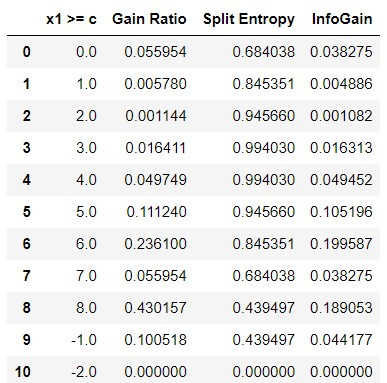
\includegraphics[width=\textwidth]{q2_3_x1.jpg}
          \caption{Information gain ratio for feature $x_1$}
          \label{fig:ig_x2}
      \end{subfigure}
      \caption{Information gain ratio for the root node state}
      \label{fig:q2_3}
  \end{figure}

\end{soln}

\item (The king of interpretability)  [10 pts] Decision tree is not the most accurate classifier in general.  However, it persists.  This is largely due to its rumored interpretability: a data scientist can easily explain a tree to a non-data scientist.  Build a tree from D3leaves.txt.  Then manually convert your tree to a set of logic rules.  Show the tree\footnote{When we say show the tree, we mean either the standard computer science tree view, or some crude plaintext representation of the tree -- as long as you explain the format.  When we say visualize the tree, we mean a plot in the 2D $\x$ space that shows how the tree will classify any points.} and the rules. \\

\begin{soln}
  The following Figure.(\ref{fig:q2_4}) shows the decision tree for the given data set. \\
  \begin{figure}[H]
    \centering
    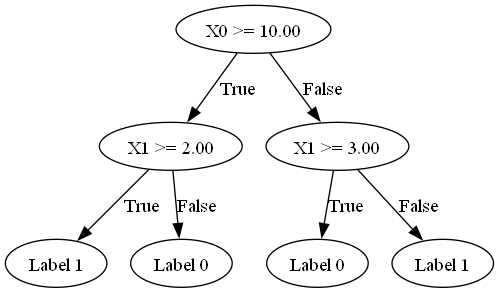
\includegraphics[width=0.5\textwidth]{d3_vis.png}
    \caption{Decision tree for D3leaves.txt}
    \label{fig:q2_4}
  \end{figure}

  The decision tree can be converted to the following set of rules,
  \begin{itemize}
    \item If $x_0 \ge 10$ and $x_1 \ge 2$ then $y=1$
    \item If $x_0 \ge 10$ and $x_1 < 2$ then $y=0$
    \item If $x_0 < 10$ and $x_1 \ge 3$ then $y=0$
    \item If $x_0 < 10$ and $x_1 < 3$ then $y=1$
  \end{itemize}

\end{soln}

\item (Or is it?)  [10 pts] For this question only, make sure you DO NOT VISUALIZE the data sets or plot your tree's decision boundary in the 2D $\x$ space.  If your code does that, turn it off before proceeding.  This is because you want to see your own reaction when trying to interpret a tree.  You will get points no matter what your interpretation is.
And we will ask you to visualize them in the next question anyway.
  \begin{itemize}
  
  \item Build a decision tree on D1.txt.  Show it to us in any format (e.g. could be a standard binary tree with nodes and arrows, and denote the rule at each leaf node; or as simple as plaintext output where each line represents a node with appropriate line number pointers to child nodes; whatever is convenient for you). Again, do not visualize the data set or the tree in the $\x$ input space.  In real tasks you will not be able to visualize the whole high dimensional input space anyway, so we don't want you to ``cheat'' here. 
  
  \item Look at your tree in the above format (remember, you should not visualize the 2D dataset or your tree's decision boundary) and try to interpret the decision boundary in human understandable English. 
  
  \item Build a decision tree on D2.txt.  Show it to us. 
  
  \item Try to interpret your D2 decision tree. Is it easy or possible to do so without visualization? \\
  
  \end{itemize}

  \begin{soln}
    The following Figure.(\ref{fig:q2_5}) shows the decision tree for D1.txt. \\
    \begin{figure}[H]
      \centering
      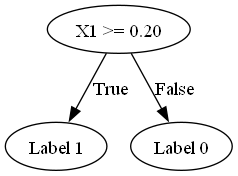
\includegraphics[width=4cm]{d1_vis.png}
      \caption{Decision tree for D1.txt}
      \label{fig:q2_5}
    \end{figure}
  
    In the decision tree for D1.txt, every data point that has its $x_1$ value greater than 0.2 is classified as 1. However, every data point that has its $x_1$ value less than 0.2 is classified as 0. It is  a very simple tree.\\

    \begin{figure}[H]
      \centering
      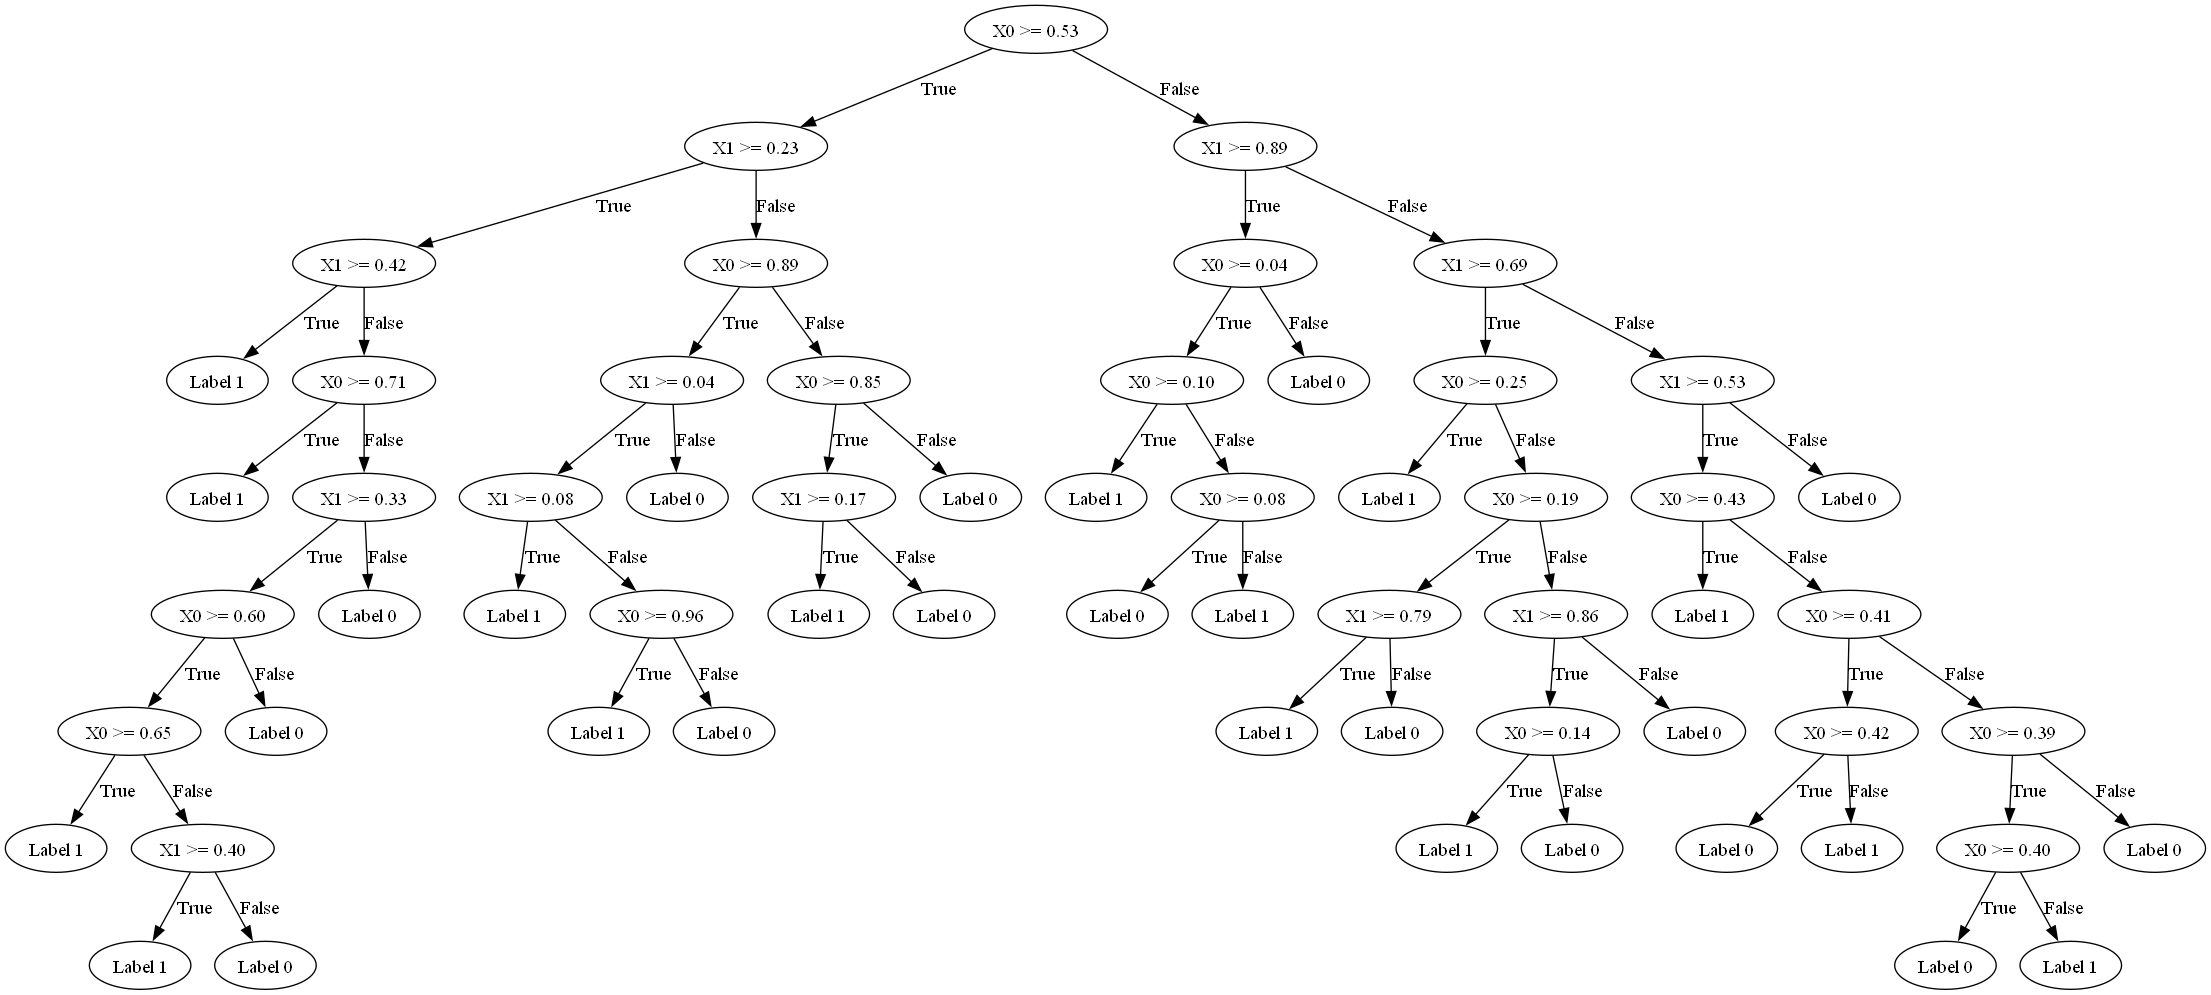
\includegraphics[width=10cm]{d2_vis.png}
      \caption{Decision tree for D2.txt}
      \label{fig:q2_6}
    \end{figure}
    
    Unlike the decision tree for D1.txt which had only three total nodes, the tree for D2.txt (Figure.\ref{fig:q2_6}) is a much complex tree with about 30 total nodes. Trying to interpret the tree by keepng track of the many branching in such a large tree is difficult. As such it is hard to get a good idea on what the decision tree is doing without the aid of visualization.
  \end{soln}

\item (Hypothesis space)  [10 pts] For D1.txt and D2.txt, do the following separately:
  \begin{itemize}
  
  \item Produce a scatter plot of the data set.

  \item Visualize your decision tree's decision boundary (or decision region, or some other ways to clearly visualize how your decision tree will make decisions in the feature space).

  \end{itemize}
Then discuss why the size of your decision trees on D1 and D2 differ.  Relate this to the hypothesis space of our decision tree algorithm. \\

\begin{soln}
  The scatter plots for D1.txt and D2.txt are as follows (Figure.\ref{fig:q2_7}),
    \begin{figure}[H]
      \centering
      \begin{subfigure}[b]{0.3\textwidth}
          \centering
          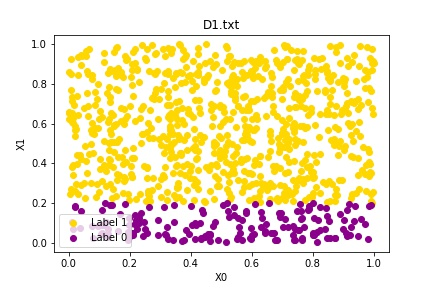
\includegraphics[width=6cm]{d1_scatter.jpg}
          \caption{Scatter plot for D1.txt}
          \label{fig:d1_scatter}
      \end{subfigure}
      \begin{subfigure}[b]{0.3\textwidth}
          \centering
          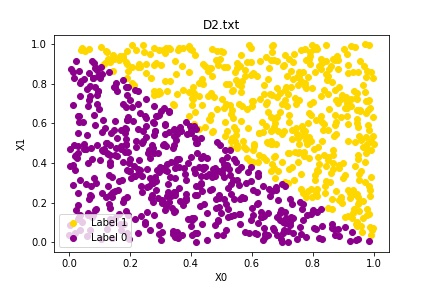
\includegraphics[width=6cm]{d2_scatter.jpg}
          \caption{Scatter plot for D2.txt}
          \label{fig:d2_scatter}
      \end{subfigure}
      \caption{Scatter plots for D1.txt and D2.txt}
      \label{fig:q2_7}
  \end{figure}


Their corresponding decision boundaries are as follows (Figure.\ref{fig:q2_8}),
\begin{figure}[H]
  \centering
  \begin{subfigure}[b]{0.3\textwidth}
      \centering
      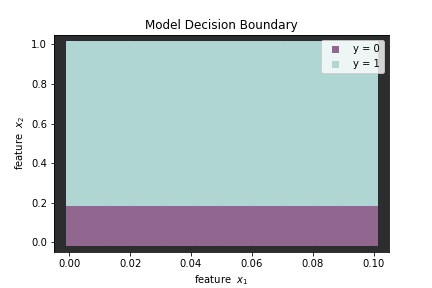
\includegraphics[width=6cm]{d1_vis_decision_boundary.png}
      \caption{Decision boundary for D1.txt}
      \label{fig:d1_vis}
  \end{subfigure}
  \begin{subfigure}[b]{0.3\textwidth}
      \centering
      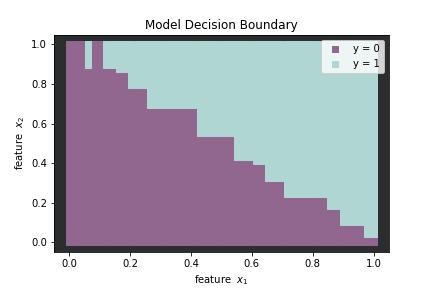
\includegraphics[width=6cm]{d2_vis_decision_boundary.png}
      \caption{Decision boundary for D2.txt}
      \label{fig:d2_vis}
  \end{subfigure}
  \caption{Decision boundaries for D1.txt and D2.txt}
  \label{fig:q2_8}
\end{figure}

The hypothesis space for our deision tree algorithm asssumes trees with single-feature and axis paralle splits. That is our decision tree tries to classify the input space by splitting it using horizontal or vertical lines based on the feature value of a single feature. According to the scatter plot of D1.txt (Figure.\ref{fig:d1_scatter}), the data is separated by a straight line. As such our decision tree can easiy separate it using a single horizontal split as seen by the decision boundary plot (Figure.\ref*{fig:d1_vis}). \\

However, the scatter plot of D2.txt (Figure.\ref{fig:d2_scatter}) shows that the data is separated by a sloped line. As such our decision tree cannot separate it using a single horizontal or vertical split. Therefore, it has to use multiple splits to separate the data. This can be seen in the decision boundary plot for D2.txt (Figure.\ref{fig:d2_vis}).This is why the decision tree for D2.txt is much larger than the decision tree for D1.txt. \\

\end{soln}


\item (Learning curve)  [20 pts] We provide a data set Dbig.txt with 10000 labeled items.  Caution: Dbig.txt is sorted.
  \begin{itemize}
  
  \item You will randomly split Dbig.txt into a candidate training set of 8192 items and a test set (the rest).  Do this by generating a random permutation, and split at 8192.
  
  \item Generate a sequence of five nested training sets $D_{32} \subset D_{128} \subset D_{512} \subset D_{2048} \subset D_{8192}$ from the candidate training set.  The subscript $n$ in $D_n$ denotes training set size.  The easiest way is to take the first $n$ items from the (same) permutation above.  This sequence simulates the real world situation where you obtain more and more training data.
  
  \item For each $D_n$ above, train a decision tree.  Measure its test set error $err_n$.  Show three things in your answer: (1) List $n$, number of nodes in that tree, $err_n$. (2) Plot $n$ vs. $err_n$.  This is known as a learning curve (a single plot). (3) Visualize your decision trees' decision boundary (five plots). \\
  \end{itemize}
  
\end{enumerate}


\begin{soln}
  \begin{itemize}
    \item [(i)] The following Table.(\ref{tab:q2_8}) lists the number of nodes in the trees,
    \begin{table}[H]
      \centering
      \begin{tabular}{|l|c|}
      \hline
      \multicolumn{1}{|c|}{$D_n$} & \textbf{Num. Nodes} \\ \hline
      $D_{32}$                               & 8                  \\ \hline
      $D_{128}$                               & 22                   \\ \hline
      $D_{512}$                               & 44                   \\ \hline
      $D_{2048}$                               & 142                  \\ \hline
      $D_{8192}$                               & 258                 \\ \hline
      \end{tabular}
      \end{table}
      \captionof{table}{Number of nodes in the decision trees}
      \label{tab:q2_8}

      \item [(ii)] The following Figure.(\ref{fig:q2_9}) shows the learning curve for the decision tree,
        \begin{figure}[H]
          \centering
          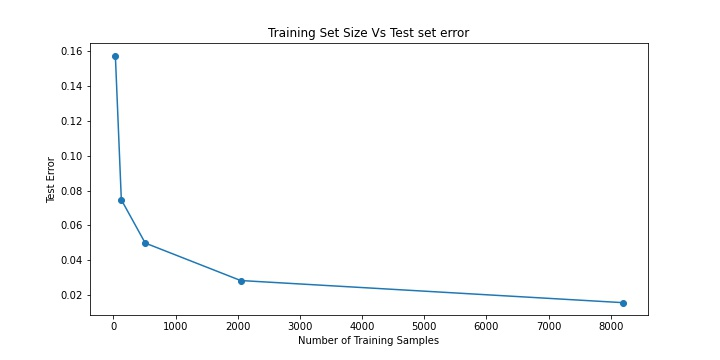
\includegraphics[width=12cm]{q27_nodes_v_err.jpg}
          \caption{Learning curve for the decision trees.}
          \label{fig:q2_9}
        \end{figure}

      \item [(iii)] The following Figures (\ref{fig:q2_12}) shows the decision boundaries for the decision trees,
        \begin{figure}[H]
          \centering
          \begin{subfigure}[b]{0.3\textwidth}
              \centering
              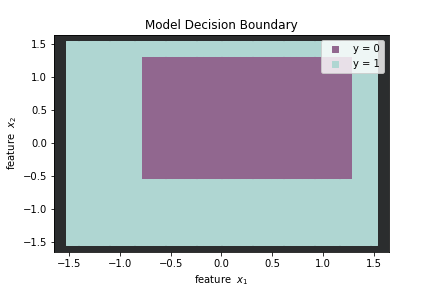
\includegraphics[width=6cm]{D32_trn_decision_boundary.png}
              \caption{Decision boundary for $D_{32}$}
              \label{fig:d32_vis}
          \end{subfigure}
          \begin{subfigure}[b]{0.3\textwidth}
              \centering
              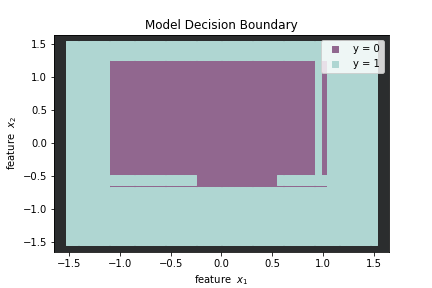
\includegraphics[width=6cm]{D128_trn_decision_boundary.png}
              \caption{Decision boundary for $D_{128}$}
              \label{fig:d128_vis}
          \end{subfigure}
          \label{fig:q2_10}
      \end{figure}


      \begin{figure}[H]
        \centering
        \begin{subfigure}[b]{0.3\textwidth}
            \centering
            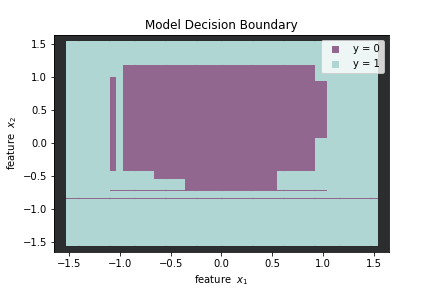
\includegraphics[width=6cm]{D512_trn_decision_boundary.png}
            \caption{Decision boundary for $D_{512}$}
            \label{fig:d32_vis}
        \end{subfigure}
        \begin{subfigure}[b]{0.3\textwidth}
            \centering
            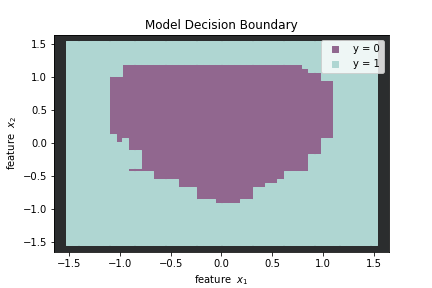
\includegraphics[width=6cm]{D2048_trn_decision_boundary.png}
            \caption{Decision boundary for $D_{2048}$}
            \label{fig:d128_vis}
        \end{subfigure}
        \label{fig:q2_11}
    \end{figure}

    \begin{figure}[H]
      \centering
      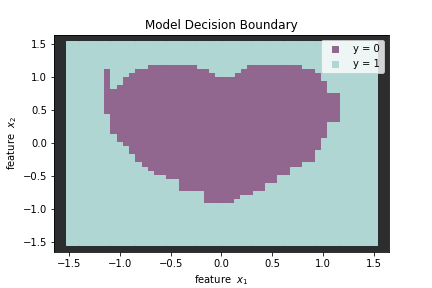
\includegraphics[width=6cm]{D8192_trn_decision_boundary.png}
      \caption{Decision boundary for $D_{8192}$}
      \label{fig:q2_12}
    \end{figure}


  \end{itemize}
\end{soln}

\section{sklearn [10 pts]}
Learn to use sklearn (\url{https://scikit-learn.org/stable/}).
Use sklearn.tree.DecisionTreeClassifier to produce trees for datasets $D_{32}, D_{128}, D_{512}, D_{2048}, D_{8192}$.  Show two things in your answer: (1) List $n$, number of nodes in that tree, $err_n$. (2) Plot $n$ vs. $err_n$.
\\
\begin{soln}
  \begin{itemize}
    \item [(i)] The following Table.(\ref{tab:q2_13}) lists the number of nodes in the trees,
    \begin{table}[H]
      \centering
      \begin{tabular}{|l|c|}
      \hline
      \multicolumn{1}{|c|}{$D_n$} & \textbf{Num. Nodes} \\ \hline
      $D_{32}$                               & 9                   \\ \hline
      $D_{128}$                               & 19                   \\ \hline
      $D_{512}$                               & 45                   \\ \hline
      $D_{2048}$                               & 133                  \\ \hline
      $D_{8192}$                               & 237                   \\ \hline
      \end{tabular}
      \end{table}
      \captionof{table}{Number of nodes in the decision trees}
      \label{tab:q2_13}


    \item [(ii)] The following Figure.(\ref{fig:q2_14}) shows the learning curve for the decision tree,
    \begin{figure}[H]
      \centering
      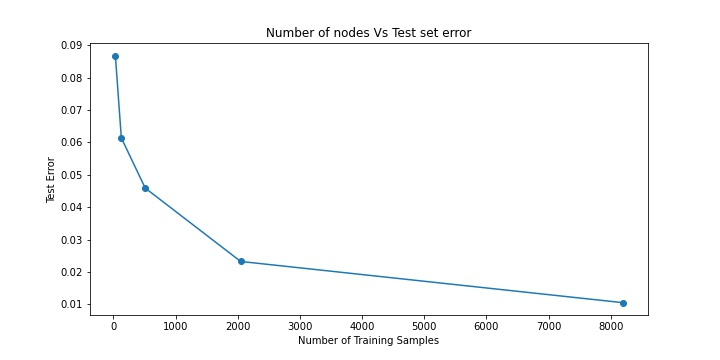
\includegraphics[width=12cm]{q3_nodes_v_err.jpg}
      \caption{Learning curve for the decision trees.}
      \label{fig:q2_14}
    \end{figure}

  \end{itemize}

\end{soln}
\section{Lagrange Interpolation [10 pts]}
Fix some interval $[a, b]$ and sample $n = 100$ points $x$ from this interval uniformly. Use these to build a training set consisting of $n$ pairs $(x, y)$ by setting function $y = sin(x)$. \\

Build a model $f$ by using Lagrange interpolation, check more details in \url{https://en.wikipedia.org/wiki/Lagrange_polynomial} and \url{https://docs.scipy.org/doc/scipy/reference/generated/scipy.interpolate.lagrange.html}. \\

Generate a test set using the same distribution as your test set. Compute and report the resulting model’s train and test error. What do you observe?
Repeat the experiment with zero-mean Gaussian noise $\epsilon$ added to $x$. Vary the standard deviation for $\epsilon$ and report your findings.

\begin{soln}
  Before adding Gaussian noise, the test set error was $\approx 6.5\mathrm{e}+64$. This is because we try to ft a lagrange polynomial using $n=100$ points. However, the lagrange interpolation is numerically unstable for $n>20$ resulting in a very high test set error. After running the same experiment with Gaussian noise of zero mean and varying standard deviation added to the training data, we see the following test set error rates (Figure.\ref{fig:q2_15}), \\

  \begin{figure}[H]
    \centering
    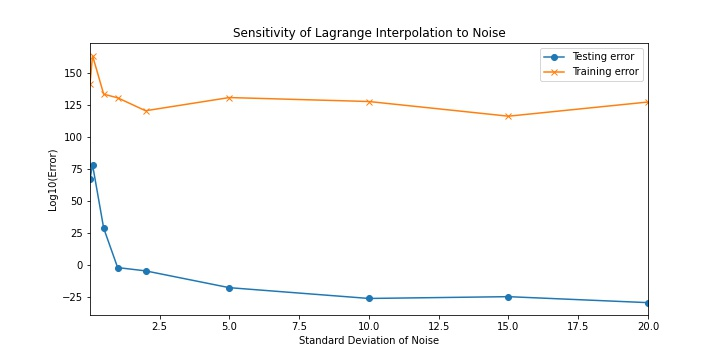
\includegraphics[width=12cm]{q4_err_plot.jpg}
    \caption{Test set error rates for added Gaussian noise with different standard deviations}
    \label{fig:q2_15}
  \end{figure}

  Even with added noise, the training set error is still very high. This is because the lagrange interpolation is numerically unstable for $n>20$. However, you can see a bit of a decreasing trend for training set error as the standard deviation of the noise increases. \\

  For a test set of $n=20$, we see that it starts off with a very high test set error but as the standard deviation of the added noise increases, the test set error decreases. With very high standard deviation, the test set error is very low, fitting the test set very well. \\
  
  % This is because the lagrange interpolation is numerically stable for $n<20$
  
\end{soln}

\bibliographystyle{apalike}
\end{document}
